% Titre : trigo
% Filiere : BCPST
% Difficulte : 
% Type : TD 
% Categories :trigo
% Subcategories : 
% Keywords : trigo




\begin{exercice}  \;
R\'esoudre sur $\R$ les \'equations suivantes et repr\'esenter les solutions sur le cercle trigonom\'etrique:\\
\begin{enumerate}
\begin{minipage}[t]{0.45\textwidth}
\item $\cos{(5x)}=\ddp\frac{\sqrt{3}}{2}$
\item $\sin{(4x)}=-\ddp\frac{1}{2}$
\end{minipage}
\begin{minipage}[t]{0.45\textwidth}
\item $\tan{\left(\ddp\frac{x}{2}\right)}=-1$
\item $\tan{(2x)}=-\sqrt{3}$
\end{minipage}
\end{enumerate}
\end{exercice}


\%\%\%\%\%\%\%\%\%\%\%\%\%\%\%\%\%\%\%\%
\%\%\%\%\%\%\%\%\%\%\%\%\%\%\%\%\%\%\%\%
\%\%\%\%\%\%\%\%\%\%\%\%\%\%\%\%\%\%\%\%




\begin{correction}  \;
Il s'agit dans cet exercice d'\'egalit\'es trigonom\'etriques fondamentales que l'on r\'esout donc en appliquant la m\'ethode du cours. 
\begin{enumerate}
 \item \textbf{R\'esolution de $\mathbf{\cos{(5x)}=\ddp\frac{\sqrt{3}}{2}}$:}
L'\'egalit\'e est de type \'equation fondamentale.
$$\begin{array}{lll}
\cos{(5x)}=\ddp\frac{\sqrt{3}}{2}&\Leftrightarrow &\cos{(5x)}= \cos{\left(\ddp\frac{\pi}{6}\right)}
\Leftrightarrow  \left\lbrace\begin{array}{l}
\exists k\in\Z,\ 5x=\ddp\frac{\pi}{6}+2k\pi\vsec\\
\hbox{ou}\vsec\\
\exists k\in\Z,\ 5x=-\ddp\frac{\pi}{6}+2k\pi.
\end{array}\right.
\end{array}$$
\begin{minipage}[c]{0.45\linewidth}
On obtient donc
\begin{equation*}
\fbox{
$\mathcal{S}=\left\lbrace \ddp\frac{\pi}{30}+\frac{2k\pi}{5},\ k\in\Z\right\rbrace\cup\left\lbrace -\ddp\frac{\pi}{30}+\frac{2k\pi}{5},\ k\in\Z\right\rbrace.$
}
\end{equation*}
\end{minipage}
\quad

\begin{center}
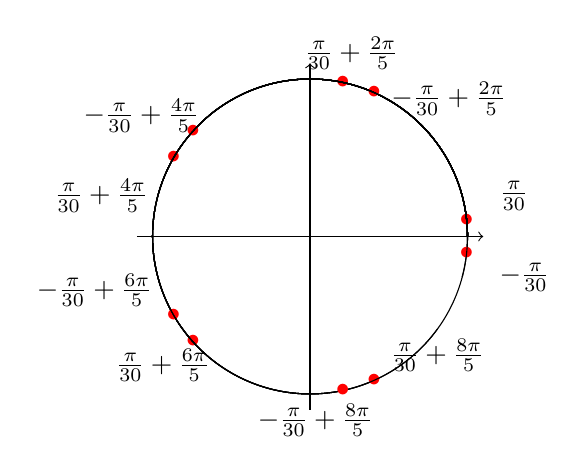
\begin{tikzpicture}[scale=2]
%Axes
\draw [->] (-1.1,0) -- (1.1,0);
\draw [->] (0,-1.1) -- (0,1.1);
%Cercle
\draw (0,0) circle (1);
%Points
\draw (1,0) arc (0:6:1) node [red] {$\bullet$};
\draw (1,0) arc (0:15:1) node[right] {$\quad \ddp \frac{\pi}{30}$} ;
\draw (1,0) arc (0:78:1) node [red] {$\bullet$};
\draw (1,0) arc (0:85:1) node[above] {$\quad\quad \ddp \frac{\pi}{30}+\frac{2\pi}{5}$} ;
\draw (1,0) arc (0:150:1) node [red] {$\bullet$};
\draw (1,0) arc (0:165:1) node[left] {$\ddp \frac{\pi}{30}+\frac{4\pi}{5}$} ;
\draw (1,0) arc (0:222:1) node [red] {$\bullet$};
\draw (1,0) arc (0:235:1) node[left] {$\ddp \frac{\pi}{30}+\frac{6\pi}{5}$} ;
\draw (1,0) arc (0:294:1) node [red] {$\bullet$};
\draw (1,0) arc (0:324:1) node[below] {$\ddp \frac{\pi}{30}+\frac{8\pi}{5}$} ;
\draw (1,0) arc (0:-6:1) node [red] {$\bullet$};
\draw (1,0) arc (0:-15:1) node[right] {$\quad \ddp - \frac{\pi}{30}$} ;
\draw (1,0) arc (0:66:1) node [red] {$\bullet$};
\draw (1,0) arc (0:45:1) node[above] {$\quad\quad \ddp -\frac{\pi}{30}+\frac{2\pi}{5}$} ;
\draw (1,0) arc (0:138:1) node [red] {$\bullet$};
\draw (1,0) arc (0:130:1) node[left] {$\ddp -\frac{\pi}{30}+\frac{4\pi}{5}$} ;
\draw (1,0) arc (0:210:1) node [red] {$\bullet$};
\draw (1,0) arc (0:200:1) node[left]  {$\ddp -\frac{\pi}{30}+\frac{6\pi}{5}$} ;
\draw (1,0) arc (0:282:1) node [red] {$\bullet$};
\draw (1,0) arc (0:272:1) node[below] {$\ddp -\frac{\pi}{30}+\frac{8\pi}{5}$} ;
\end{tikzpicture}
\end{center}

Pour savoir combien de points tracer sur le cercle pour chaque ensemble de solutions, on cherche la premi\`ere valeur de $k$ pour laquelle on retombe sur la solution de d\'epart modulo $2\pi$. Par exemple, pour le premier ensemble de solution, on cherche $k$ tel que $\ddp \frac{2k\pi}{5} = 2\pi$, soit $k=5$ : on doit donc tracer $5$ points sur le cercle trigonom\'etrique. M\^eme chose pour le deuxi\`eme ensemble de solutions.
%------------------------------
\item  \textbf{R\'esolution de $\mathbf{\sin{(4x)}=-\ddp\frac{1}{2}}$:}
L'\'egalit\'e est de type \'equation fondamentale.
$$\begin{array}{lll}
\sin{(4x)}=-\ddp\frac{1}{2}&\Leftrightarrow &\sin{(4x)}= \sin{\left(-\ddp\frac{\pi}{6}\right)}
\Leftrightarrow  \left\lbrace\begin{array}{l}
\exists k\in\Z,\ 4x=-\ddp\frac{\pi}{6}+2k\pi\vsec\\
\hbox{ou}\vsec\\
\exists k\in\Z,\ 4x=\pi+\ddp\frac{\pi}{6}+2k\pi.
\end{array}\right.
\end{array}$$
\begin{minipage}[c]{0.45\linewidth}
On obtient donc
\begin{equation*}
\fbox{
$\mathcal{S}=\left\lbrace -\ddp\frac{\pi}{24}+\frac{k\pi}{2},\ k\in\Z\right\rbrace\cup\left\lbrace \ddp\frac{7\pi}{24}+\frac{k\pi}{2},\ k\in\Z\right\rbrace.$
}
\end{equation*}
\end{minipage}
\quad

\begin{center}
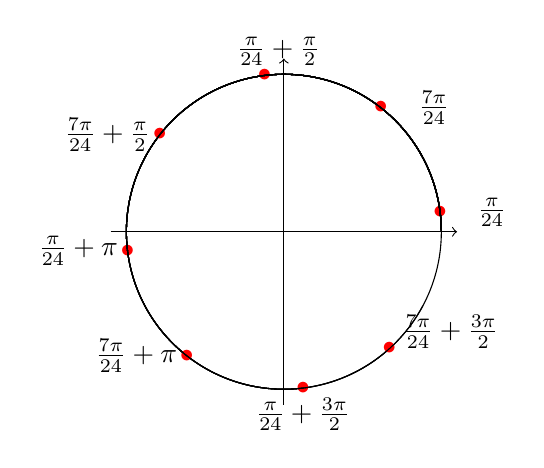
\begin{tikzpicture}[scale=2]
%Axes
\draw [->] (-1.1,0) -- (1.1,0);
\draw [->] (0,-1.1) -- (0,1.1);
%Cercle
\draw (0,0) circle (1);
%Points
\draw (1,0) arc (0:7:1) node [red] {$\bullet$};
\draw (1,0) arc (0:7:1) node[right] {$\quad \ddp \frac{\pi}{24}$} ;
\draw (1,0) arc (0:97:1) node [red] {$\bullet$};
\draw (1,0) arc (0:97:1) node[above] {$\quad \ddp \frac{\pi}{24}+\frac{\pi}{2}$} ;
\draw (1,0) arc (0:187:1) node [red] {$\bullet$};
\draw (1,0) arc (0:187:1) node[left] {$\ddp \frac{\pi}{24}+\pi$} ;
\draw (1,0) arc (0:277:1) node [red] {$\bullet$};
\draw (1,0) arc (0:277:1) node[below] {$\ddp \frac{\pi}{24}+\frac{3\pi}{2}$} ;
\draw (1,0) arc (0:52:1) node [red] {$\bullet$};
\draw (1,0) arc (0:52:1) node[right] {$\quad \ddp \frac{7\pi}{24}$} ;
\draw (1,0) arc (0:142:1) node [red] {$\bullet$};
\draw (1,0) arc (0:142:1) node[left] {$\quad \ddp \frac{7\pi}{24}+\frac{\pi}{2}$} ;
\draw (1,0) arc (0:232:1) node [red] {$\bullet$};
\draw (1,0) arc (0:232:1) node[left] {$\quad \ddp \frac{7\pi}{24}+\pi$} ;
\draw (1,0) arc (0:312:1) node [red] {$\bullet$};
\draw (1,0) arc (0:332:1) node[below]  {$\quad \quad \ddp \frac{7\pi}{24}+\frac{3\pi}{2}$} ;
\end{tikzpicture}
\end{center}

On remarque ici qu'il faut tracer $4$ points pour chaque ensemble de solutions : en effet, on doit chercher $k$ tel que $\ddp \frac{k \pi}{2} = 2 \pi$, soit $k=4$.
%-------------------------------------
\item \textbf{R\'esolution de $\mathbf{\tan{\left(\ddp\frac{x}{2}\right)}}$:}
L'\'egalit\'e est de type \'equation fondamentale. On peut commencer par chercher le domaine de d\'efinition de cette \'equation. On a, d'apr\`{e}s le domaine de d\'efinition de la tangente, que: $\ddp\frac{x}{2}\not= \ddp\frac{\pi}{2}+k\pi,\ k\in\Z\Leftrightarrow x\not= \pi+2k\pi,\ k\in\Z$. On r\'esout ensuite l'\'equation fondamentale et on v\'erifiera bien que les solutions trouv\'ees n'appartiennent pas \`{a} l'ensemble $\left\lbrace  \pi+2k\pi,\ k\in\Z \right\rbrace$. 
$$\begin{array}{lll}
\tan{\left(\ddp\frac{x}{2}\right)}=-1 &\Leftrightarrow & \tan{\left(\ddp\frac{x}{2}\right)}= \tan{\left(-\ddp\frac{\pi}{4}\right)}
\Leftrightarrow  \exists k\in\Z,\ \ddp\frac{x}{2}=-\ddp\frac{\pi}{4}+k\pi.\\
%&\Leftrightarrow & \begin{array}{|l|}
%\hline
%\exists k\in\Z,\ x=-\ddp\frac{\pi}{2}+2k\pi.\\
%\hline
%\end{array}
\end{array}$$
On obtient donc
\begin{equation*}
\fbox{
$\mathcal{S}=\left\lbrace -\ddp\frac{\pi}{2}+2k\pi,\ k\in\Z\right\rbrace.$
}
\end{equation*}
%-------------------------------------
\item \textbf{R\'esolution de $\mathbf{ \tan{(2x)}=-\sqrt{3}}$:}
L'\'egalit\'e est de type \'equation fondamentale.
On peut commencer par chercher le domaine de d\'efinition de cette \'equation. On a, d'apr\`{e}s le domaine de d\'efinition de la tangente, que: $2x\not= \ddp\frac{\pi}{2}+k\pi,\ k\in\Z\Leftrightarrow x\not= \ddp\frac{\pi}{4}+\ddp\frac{k\pi}{2} ,\ k\in\Z$. On r\'esout ensuite l'\'equation fondamentale et on v\'erifiera bien que les solutions trouv\'ees n'appartiennent pas \`{a} l'ensemble $\left\lbrace \ddp\frac{\pi}{4}+\ddp\frac{k\pi}{2},\ k\in\Z \right\rbrace$. 
$$\begin{array}{lll}
\tan{(2x)}=-\sqrt{3} &\Leftrightarrow & \tan{(2x)}= \tan{\left(-\ddp\frac{\pi}{3}\right)}
\Leftrightarrow  \exists k\in\Z,\ 2x=-\ddp\frac{\pi}{3}+k\pi.
\end{array}$$
\begin{minipage}[c]{0.45\linewidth}
On obtient donc
\begin{equation*}
\fbox{
$\mathcal{S}=\left\lbrace -\ddp\frac{\pi}{6}+\ddp\frac{k\pi}{2},\ k\in\Z\right\rbrace.$
}
\end{equation*}
\end{minipage}
\quad
\begin{minipage}[c]{0.45\linewidth}
\begin{center}
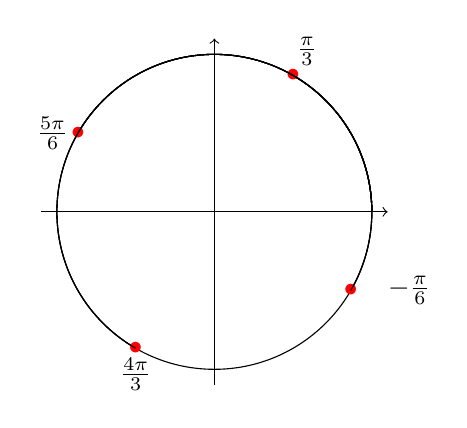
\begin{tikzpicture}[scale=2]
%Axes
\draw [->] (-1.1,0) -- (1.1,0);
\draw [->] (0,-1.1) -- (0,1.1);
%Cercle
\draw (0,0) circle (1);
%Points
\draw (1,0) arc (0:-30:1) node [red] {$\bullet$};
\draw (1,0) arc (0:-30:1) node[right] {$\quad \ddp -\frac{\pi}{6}$} ;
\draw (1,0) arc (0:60:1) node [red] {$\bullet$};
\draw (1,0) arc (0:60:1) node[above] {$\quad \ddp \frac{\pi}{3}$} ;
\draw (1,0) arc (0:150:1) node [red] {$\bullet$};
\draw (1,0) arc (0:150:1) node[left] {$\ddp \frac{5\pi}{6}$} ;
\draw (1,0) arc (0:240:1) node [red] {$\bullet$};
\draw (1,0) arc (0:240:1) node[below] {$\ddp \frac{4\pi}{3}$} ;
\end{tikzpicture}
\end{center}
\end{minipage}
\end{enumerate}
\end{correction}